\documentclass[landscape,final,a0paper,fontscale=0.33]{baposter}
% suppress warnings when running from command line `pdflatex chasm_poster`
% Or, include this package:
\usepackage{silence}
\WarningsOff*

%\nonstopmode

\usepackage{calc}
\usepackage{graphicx}
\usepackage{amsmath}
\usepackage{amssymb}
\usepackage{relsize}
\usepackage{multirow}
\usepackage{rotating}
\usepackage{bm}
\usepackage{url}
\usepackage{color}
\usepackage{graphicx}
\usepackage{epsfig}
\usepackage{multicol}
\usepackage{smile}
\usepackage{sans}
\usepackage{float}
\usepackage[ruled]{algorithm2e}
\usepackage[font=scriptsize]{caption}
\usepackage{wrapfig}
\usepackage[normalem]{ulem}
%\usepackage{decorations}
\usetikzlibrary{decorations}
%\usetikzlibrary{decorations.pathmorphing}
%\usepackage{algorithm}

%\sbox0{\sffamily x}
%\DeclareFontShape{T1}{cmss}{bx}{sc}{<->ssub*cmss/bx/n}{}
%\usepackage[T1]{fontenc}
%\usepackage[ansinew]{inputenc}

%\SetAlgoCaptionSeparator{.}
%\renewcommand\AlCapFnt{\scriptsize\scshape}
%\captionsetup[algorithm2e]{font=scriptsize}

%\usepackage{times}
%\usepackage{helvet}
%\usepackage{bookman}
%\usepackage{palatino}

%\newcommand{\captionfont}{\footnotesize}

%%%%%%%%%%%%%%%%%%%%%%%%%%%%%%%%%%%%%%%%%%%%%%%%%%%%%%%%%%%%%%%%%%%%%%%%%%%%%%%%
%%%% Some math symbols used in the text
%%%%%%%%%%%%%%%%%%%%%%%%%%%%%%%%%%%%%%%%%%%%%%%%%%%%%%%%%%%%%%%%%%%%%%%%%%%%%%%%

%%%%%%%%%%%%%%%%%%%%%%%%%%%%%%%%%%%%%%%%%%%%%%%%%%%%%%%%%%%%%%%%%%%%%%%%%%%%%%%%
% Multicol Settings
%%%%%%%%%%%%%%%%%%%%%%%%%%%%%%%%%%%%%%%%%%%%%%%%%%%%%%%%%%%%%%%%%%%%%%%%%%%%%%%%
\setlength{\columnsep}{1.5em}
\setlength{\columnseprule}{0mm}

%%%%%%%%%%%%%%%%%%%%%%%%%%%%%%%%%%%%%%%%%%%%%%%%%%%%%%%%%%%%%%%%%%%%%%%%%%%%%%%%
% Save space in lists. Use this after the opening of the list
%%%%%%%%%%%%%%%%%%%%%%%%%%%%%%%%%%%%%%%%%%%%%%%%%%%%%%%%%%%%%%%%%%%%%%%%%%%%%%%%
\newcommand{\compresslist}{%
\setlength{\itemsep}{1pt}%
\setlength{\parskip}{0pt}%
\setlength{\parsep}{0pt}%
}

%%%%%%%%%%%%%%%%%%%%%%%%%%%%%%%%%%%%%%%%%%%%%%%%%%%%%%%%%%%%%%%%%%%%%%%%%%%%%%
%%% Begin of Document
%%%%%%%%%%%%%%%%%%%%%%%%%%%%%%%%%%%%%%%%%%%%%%%%%%%%%%%%%%%%%%%%%%%%%%%%%%%%%%

\begin{document}
% Define some colors
\definecolor{maroon}{RGB}{123,17,19}
\definecolor{red}{RGB}{255, 0, 0}

\newcommand{\SSfontsize}{}
\hyphenation{resolution occlusions}
%%
\begin{poster}%
  % Poster Options
  {
  % Show grid to help with alignment
  grid=false,
  % Column spacing
  colspacing=1em,
  % Color style
  bgColorOne=white,
  bgColorTwo=white,
  borderColor=maroon,
  headerColorOne=black,
  headerColorTwo=maroon,
  headerFontColor=white,
  boxColorOne=white,
  boxColorTwo=maroon,
  % Format of textbox
  textborder=roundedleft,
  % Format of text header
  eyecatcher=true,
  headerborder=closed,
  headerheight=0.1\textheight,
%  textfont=\sc, An example of changing the text font
  headershape=roundedright,
  headershade=shadelr,
  headerfont=\large\bf\textsc, %Sans Serif
  textfont={\setlength{\parindent}{1.5em}},
  boxshade=plain,
%  background=shade-tb,
  background=plain,
  linewidth=2pt,
  columns=3
  }
  % Eye Catcher
  {
\includegraphics[scale = 0.5]{logo-eps-converted-to}}
  % Title
  {\hspace{1.5em}\huge\bf\textsc{Single \ \ Pixel \ \ Thermal \ \ Imaging \ \ via \ \ Adaptive \ \ Sampling}\vspace{0.2em}}
  % Authors
  {\hspace{2em}Scott Sievert (sieve121@umn.edu) and Jarvis Haupt (jdhaupt@umn.edu) \\ \hspace{2em}\large{Department of Electrical and Computer Engineering, University of Minnesota , Twin Cities, Minneapolis, MN 55455, USA}}
  % University logo
 {% The makebox allows the title to flow into the logo, this is a hack because of the L shaped logo.
     %\hspace{-0.1em}
\includegraphics[scale = 0.7]{name-eps-converted-to}
     \hspace{-0.1em}
\includegraphics[scale = 0.4]{wordmark}
  }

%%%%%%%%%%%%%%%%%%%%%%%%%%%%%%%%%%%%%%%%%%%%%%%%%%%%%%%%%%%%%%%%%%%%%%%%%%%%%%
%%% Now define the boxes that make up the poster
%%%---------------------------------------------------------------------------
%%% Each box has a name and can be placed absolutely or relatively.
%%% The only inconvenience is that you can only specify a relative position
%%% towards an already declared box. So if you have a box attached to the
%%% bottom, one to the top and a third one which should be in between, you
%%% have to specify the top and bottom boxes before you specify the middle
%%% box.
%%%%%%%%%%%%%%%%%%%%%%%%%%%%%%%%%%%%%%%%%%%%%%%%%%%%%%%%%%%%%%%%%%%%%%%%%%%%%%
    %
    % A coloured circle useful as a bullet with an adjustably strong filling
    %\newcommand{\colouredcircle}{%
      %%\tikz{\useasboundingbox (-0.2em,-0.32em) rectangle(0.2em,0.32em); \draw[draw=black,fill=lightblue,line width=0.03em] (0,0) circle(0.18em);}}
    %*}

% OUTLINE (UNWRAP)
%%%%%% COL 1
%   abstract
%   motivation
%       thermal imaging has applications in...
%   approach
%       single pixel adaptive sensor
%       hardware device
%       use haar wavelet domain
%%%%%% COL 2
%   method
%       non-zero wavelet coefficients
%   hardware
%%%%%% COL 3
%   experimental results
%       exhaustive sampling
%   conclusions/next steps
%       package hardware
%       compare with other approaches (cite Rob/Becca paper)
%   Refs, Ack

  %%% COLUMN 1
\headerbox{Abstract}{name=overview,column=0,row=0}{
    \noindent \SSfontsize{We describe a novel approach to long-wavelength infrared imaging, or \emph{thermal imaging}.  We exploit an agile architecture with a single low-cost thermal sensor that can be independently actuated in two dimensions to collect narrow field-of-view spatial ``samples'' of the scene of interest, equipping it with a simple \emph{adaptive sensing} methodology to guide the sampling process toward spatial regions of interest, to effectively produce high-resolution thermal images from relatively few samples.  We provide experimental evaluations to demonstrate the viability of our approach.
    %A sampling strategy is presented that adaptively samples using information from the wavelet domain to select where to sample next. There are many benefits to such an adaptive sampling strategy such as system cost. There are other adaptive sensing strategies but the wavelet basis simplifies the problem.
    }
    \vspace{0.4em}
}
\headerbox{Background}{name=background,column=0,below=overview}{%,above=bottom}{
\noindent \SSfontsize{Some Thermal Imaging Preliminaries:
\begin{itemize}
\item All objects with temperatures above absolute zero emit electromagnetic radiation (according to the \emph{black body radiation} law).
\item The ``peak'' wavelength at which energy is emitted decreases with increasing object temperature.
\item Objects having temperatures between about 0$^{\circ}$C and 100$^{\circ}$C emit their peak energies at wavelengths in the \emph{long-wavelength infrared} regime ($\sim$8000-15000nm), much longer than the wavelengths of visible light ($\sim$400-700nm).
\item Long-wavelength IR imaging (aka \emph{thermal imaging}) has emerged as a valuable tool with residential, industrial, and medical applications (see Figure~\ref{cc} below).
\end{itemize}


        \begin{center}
        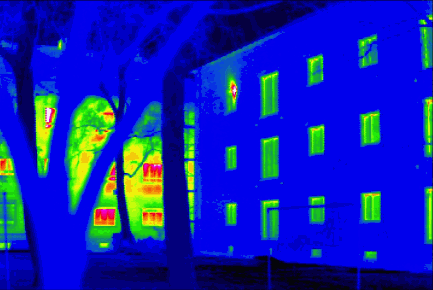
\includegraphics[height=0.15\textwidth]{figures/wiki1} \ \ \ \
        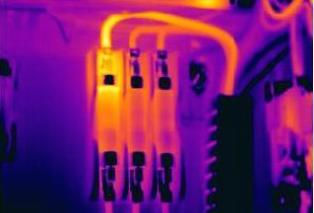
\includegraphics[height=0.15\textwidth]{figures/wiki22} \ \ \ \
        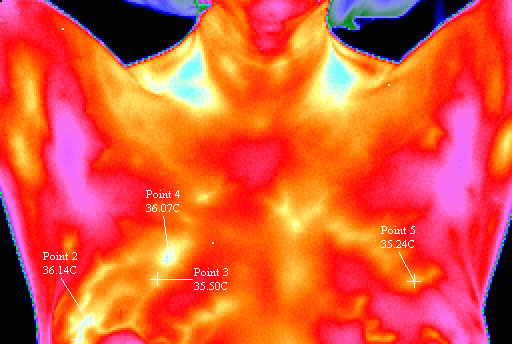
\includegraphics[height=0.15\textwidth]{figures/wiki3}
        \captionof{figure}{Thermal images can indicate residential heat losses, industrial faults, and even certain cancers. (\emph{images from Wikipedia})}\label{cc}
        \end{center}


            }
}
\headerbox{Problem Statement \& Our Approach}{name=our,column=0,row=2, below=background, above = bottom}{
    \noindent \SSfontsize{Low-cost visible light sensors (e.g., CMOS and CCD) are \uline{\textbf{not}} receptive to long-wavelength IR radiation. Instead, thermal imaging systems require expensive sensors and can cost upwards of \$3,000 or more to produce high resolution images!\\
\\
We develop an alternative approach that uses a \emph{single} steerable long-wavelength IR sensor capable of ``sampling'' at user-specified points in the scene, and is equipped with a multi-stage \emph{adaptive sensing} strategy designed to \emph{automatically} acquire only ``informative'' samples of the scene.\\
\\
\uline{Enabling idea}: \emph{Edges} often convey most information in (thermal) images.\\
\\
Our adaptive sensing approach (described next) exploits the fact that edge detail is naturally ``unveiled'' by the multi scale (Haar) wavelet representation of the image (see, e.g., Figure~\ref{multi} below)

    \begin{center}
        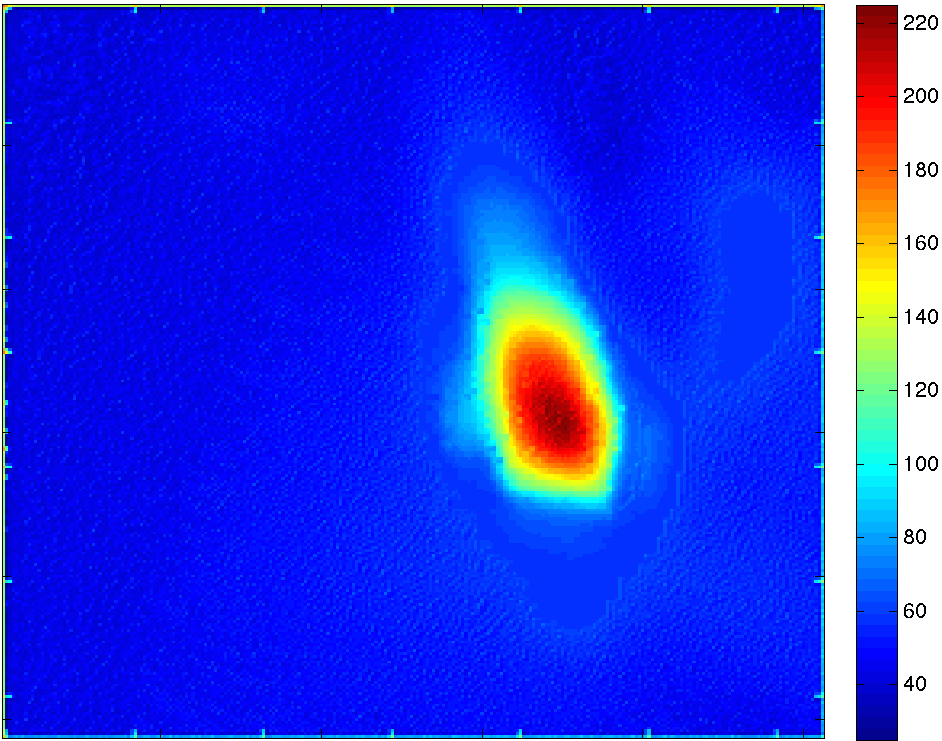
\includegraphics[width=0.16\textwidth]{figures/p} {\footnotesize =}
        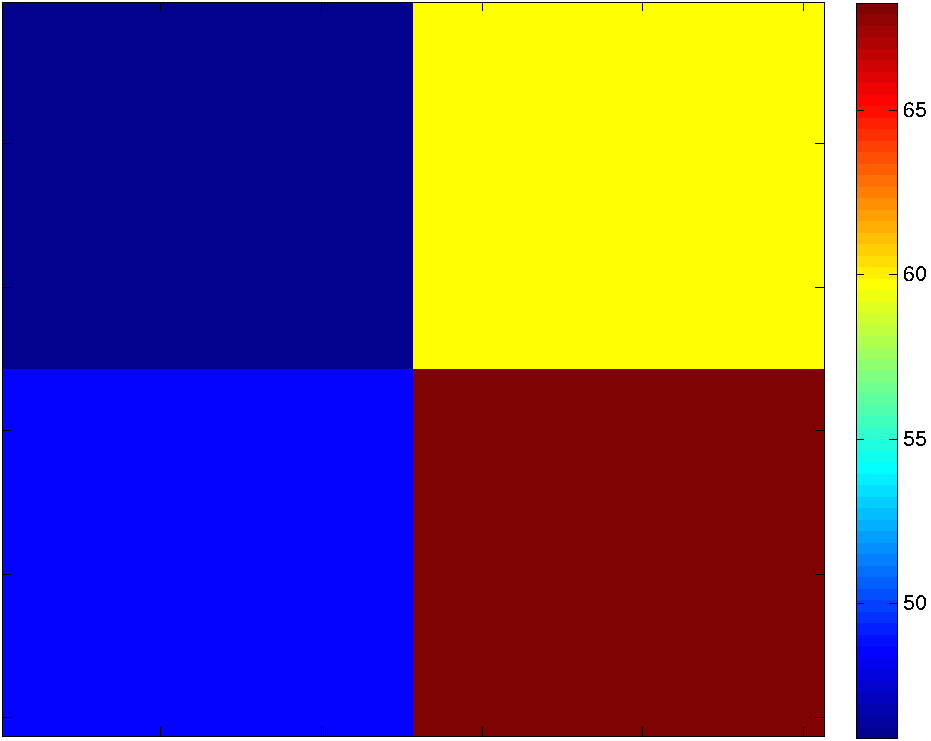
\includegraphics[width=0.16\textwidth]{figures/p1} {\footnotesize +}
        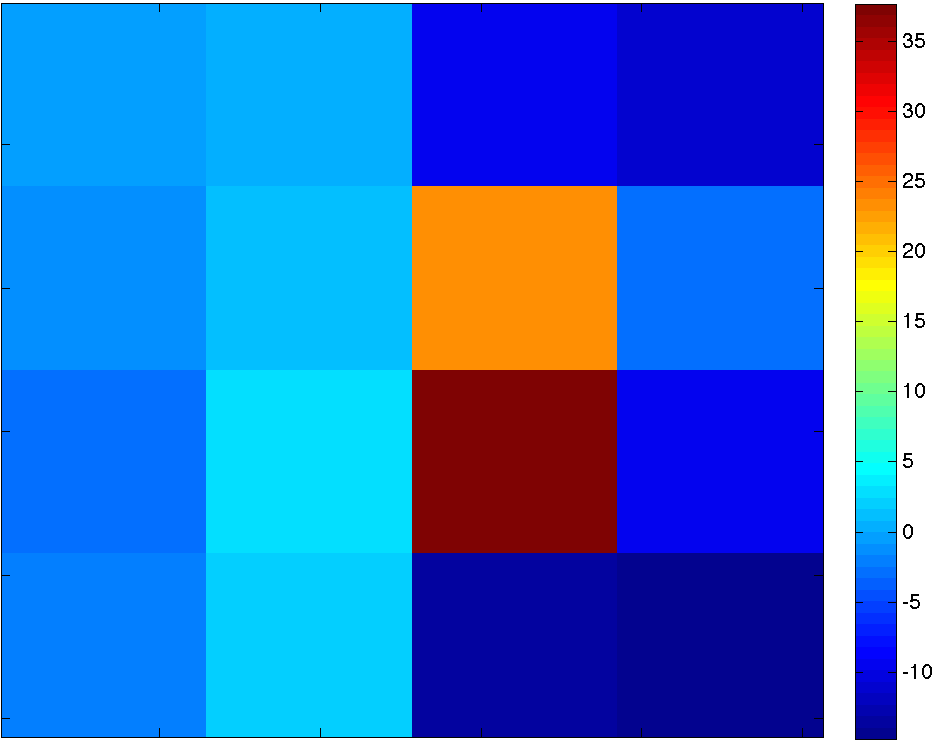
\includegraphics[width=0.16\textwidth]{figures/p2} {\footnotesize +}
        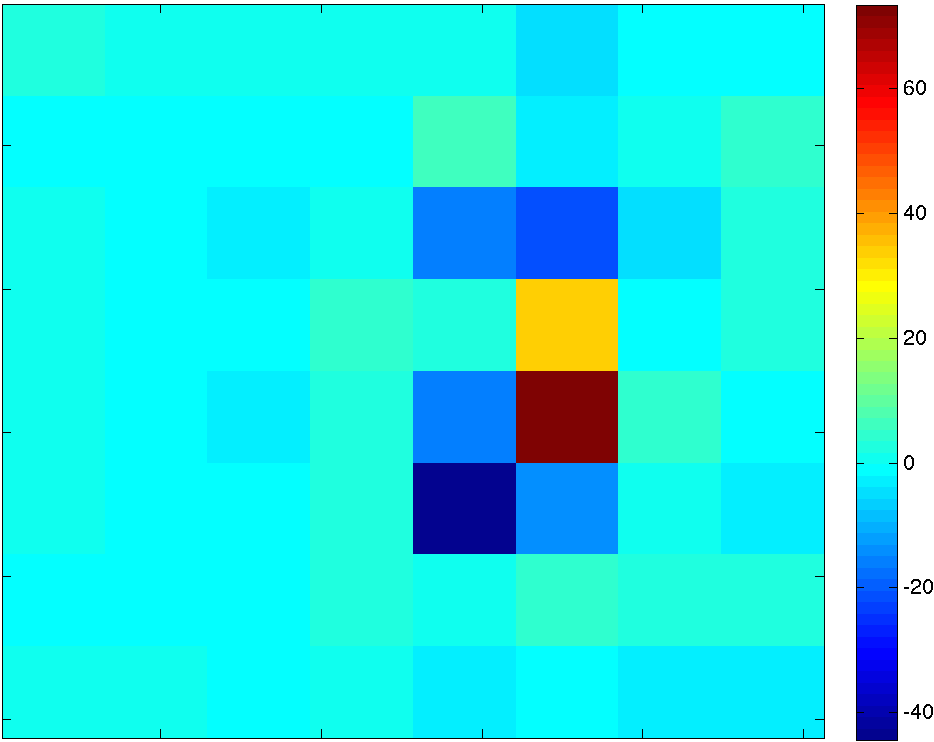
\includegraphics[width=0.16\textwidth]{figures/p3} {\footnotesize +}
         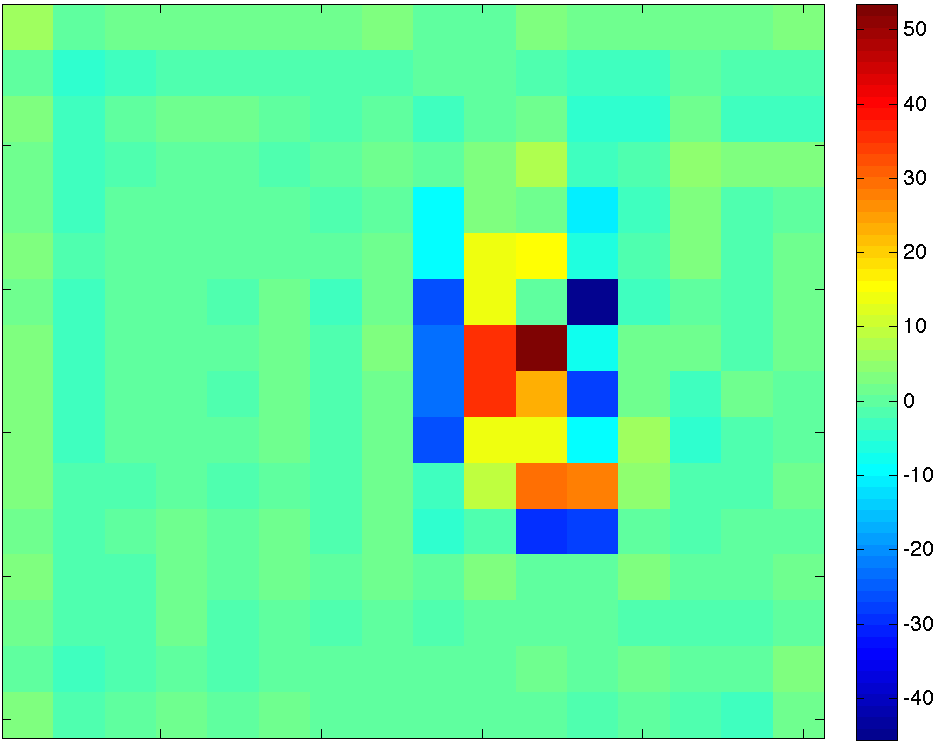
\includegraphics[width=0.16\textwidth]{figures/p4} {\footnotesize +...}
        \captionof{figure}{Multiresolution (Haar) decomposition of a thermal image (far left).  Contributions at increasingly finer scales (moving from left to right) are restricted essentially to the vicinity of \emph{edges} in the original image.}\label{multi}
        \end{center}



    }
}


  %%% COLUMN 2
\headerbox{Adaptive Sensing Methodology}{name=recon,column=1, row=0}{%,below = top, above = bottom}{
    \noindent  \SSfontsize{
%        Using this single pixel sensor we want to sample at areas that contain the most detail to reconstruct the most accurate approximation. The camera looks for edges in the Haar wavelet domain and reconstructs a wavelet approximation.
%
%        \begin{minipage}{0.48\textwidth}
%        Some text here...
%%\begin{figure}[H]
%%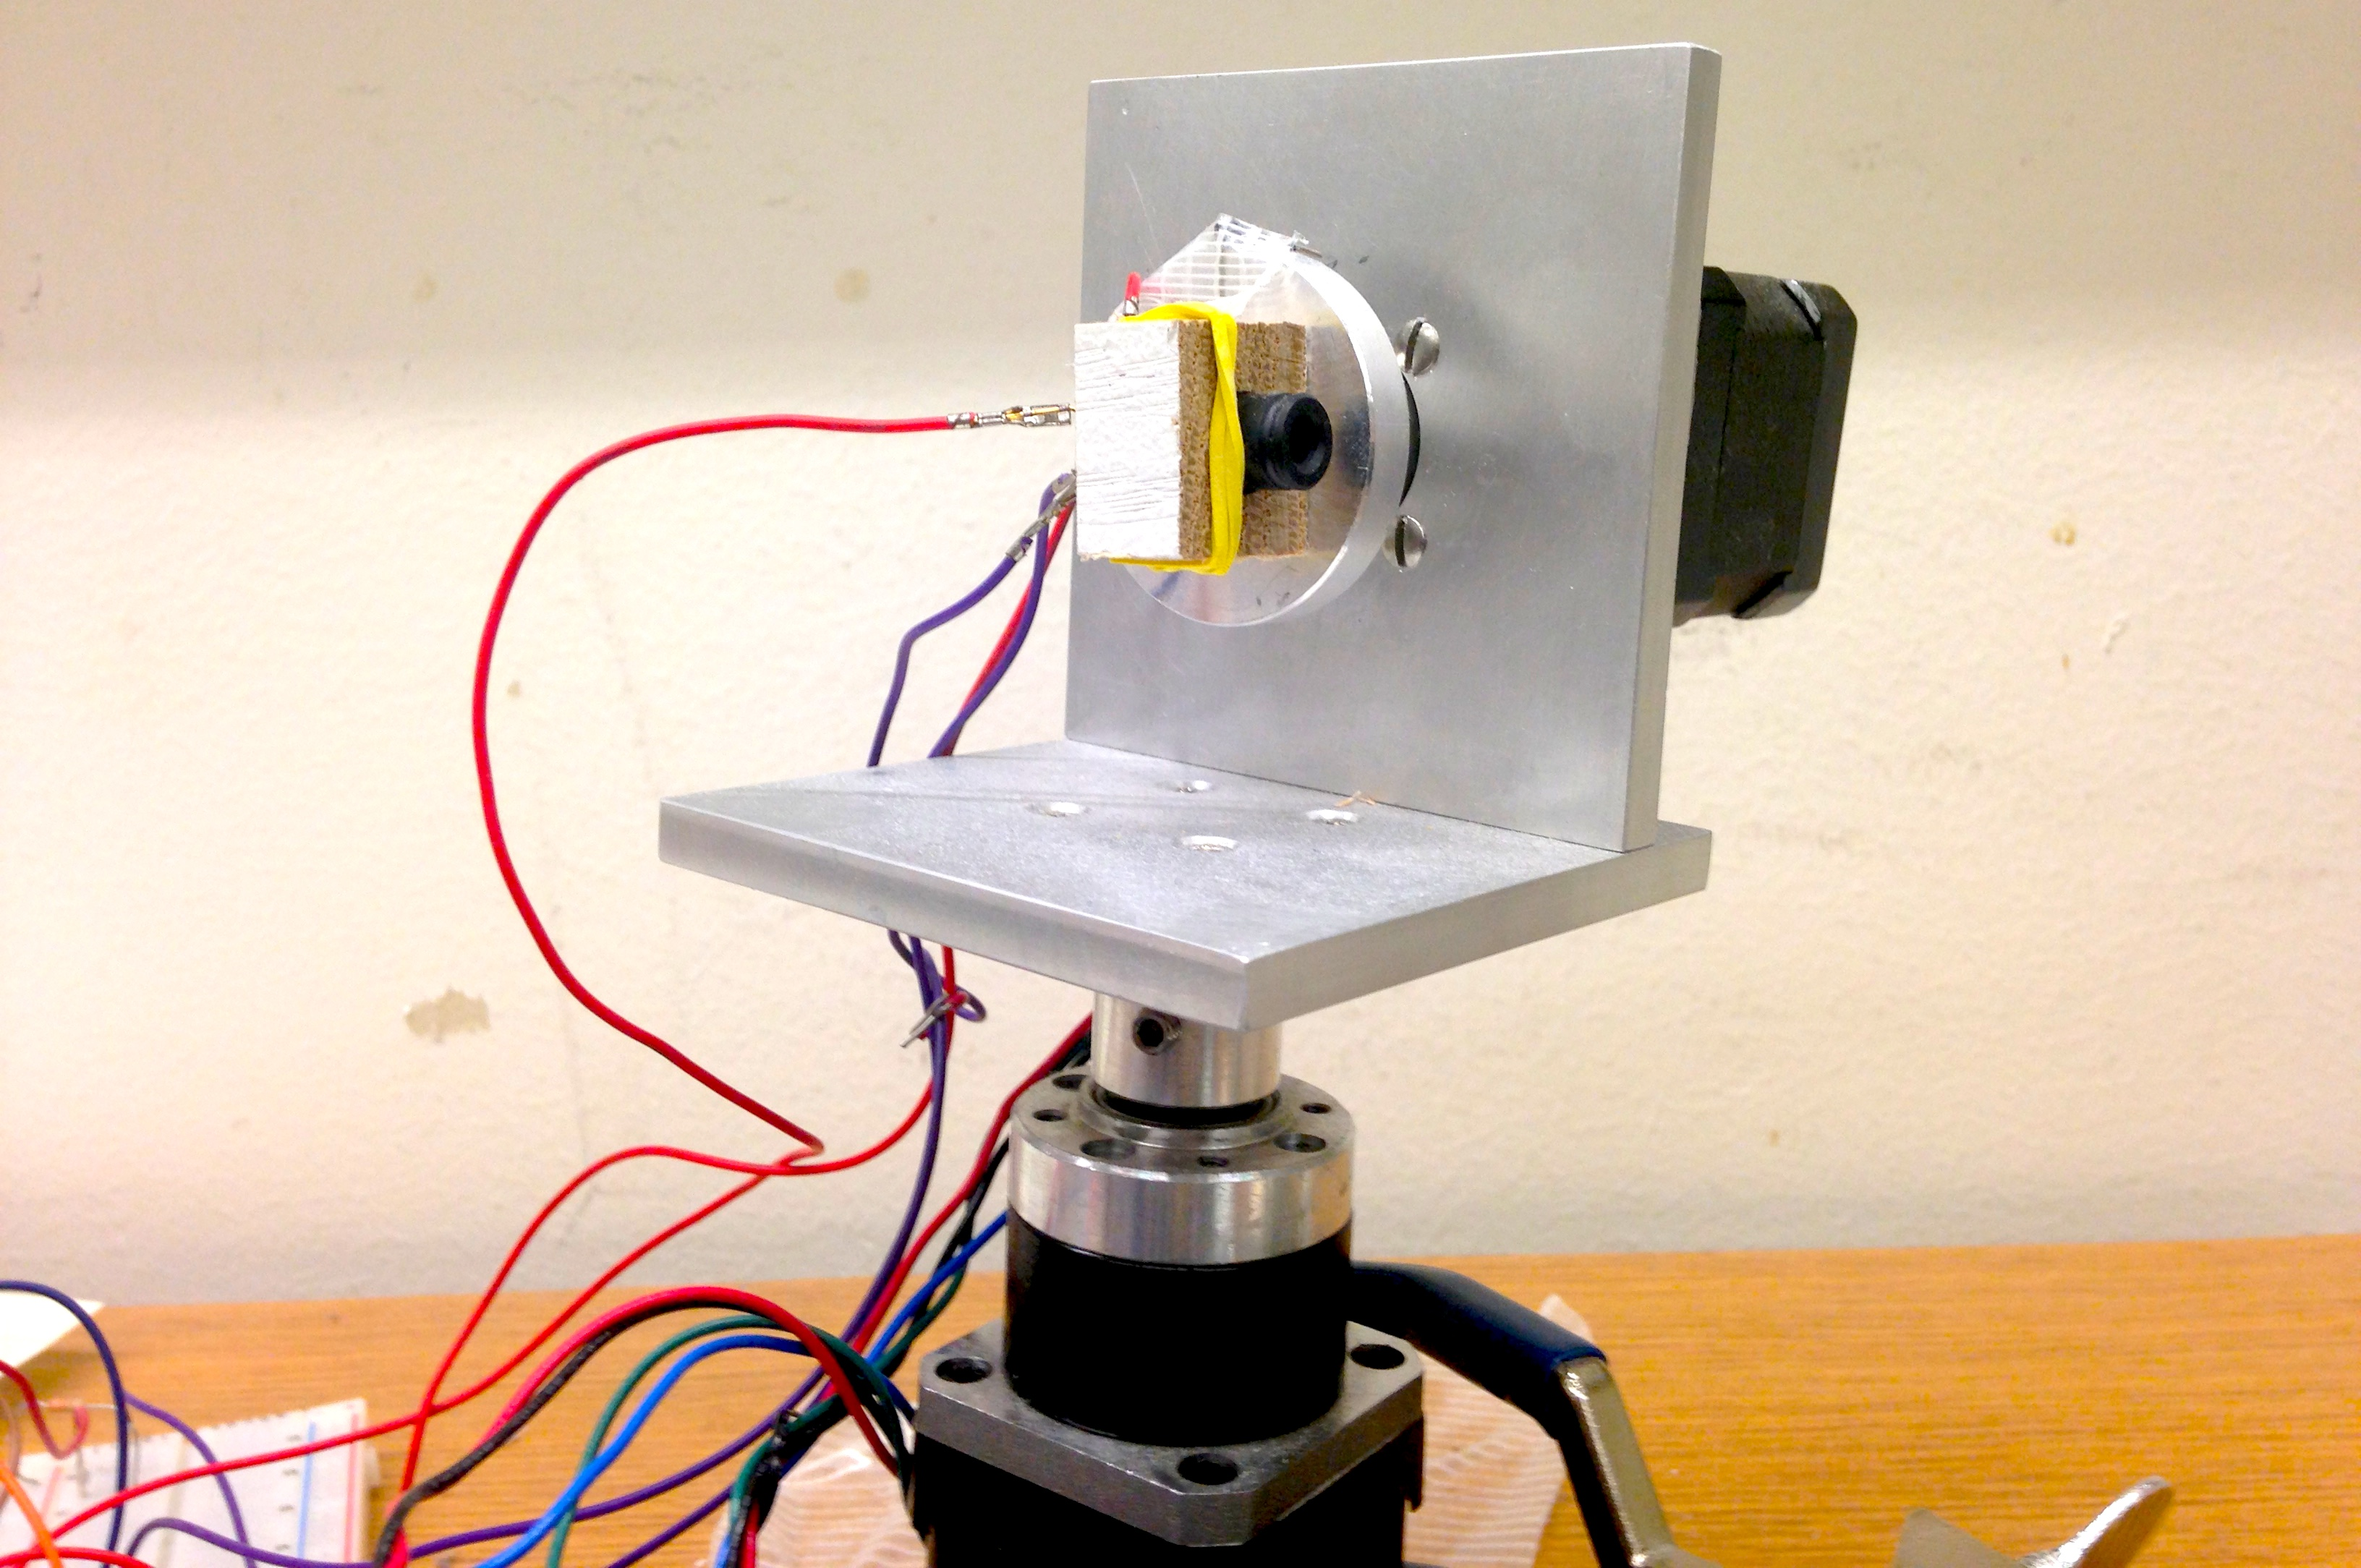
\includegraphics[width=0.95\textwidth]{figures/hardware_real}
%%\captionof{figure}{Image sensor and stepper motor assembly.}\label{cam}%\caption{\label{cam} The image sensor and stepper motor assembly.}
%%\end{figure}
%\end{minipage} \hspace{1em}
%\begin{minipage}{0.45\textwidth}
%%\begin{figure}
%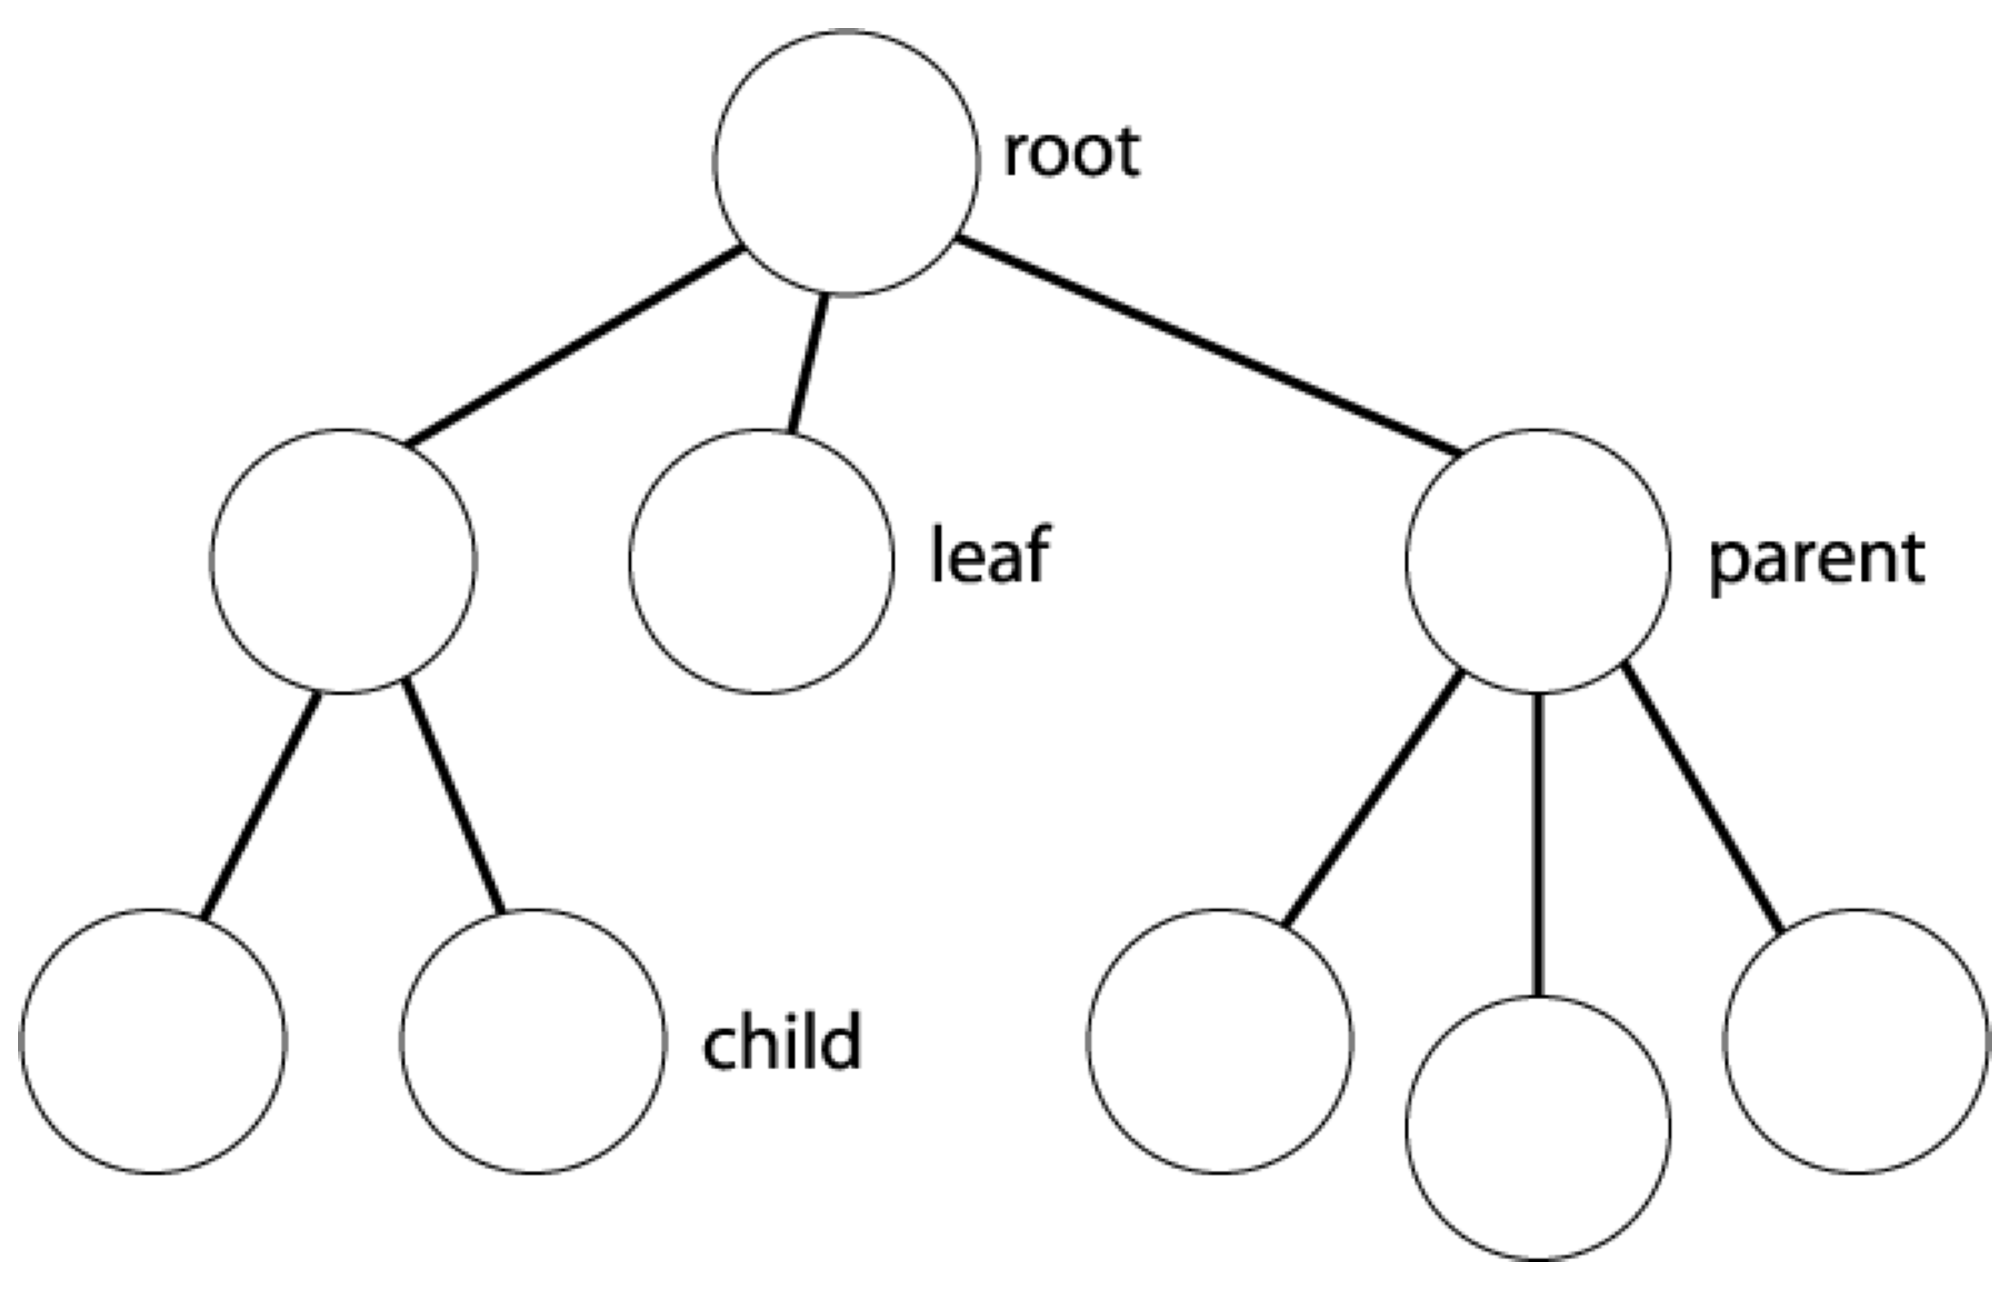
\includegraphics[width=0.9\textwidth]{figures/tree}
%%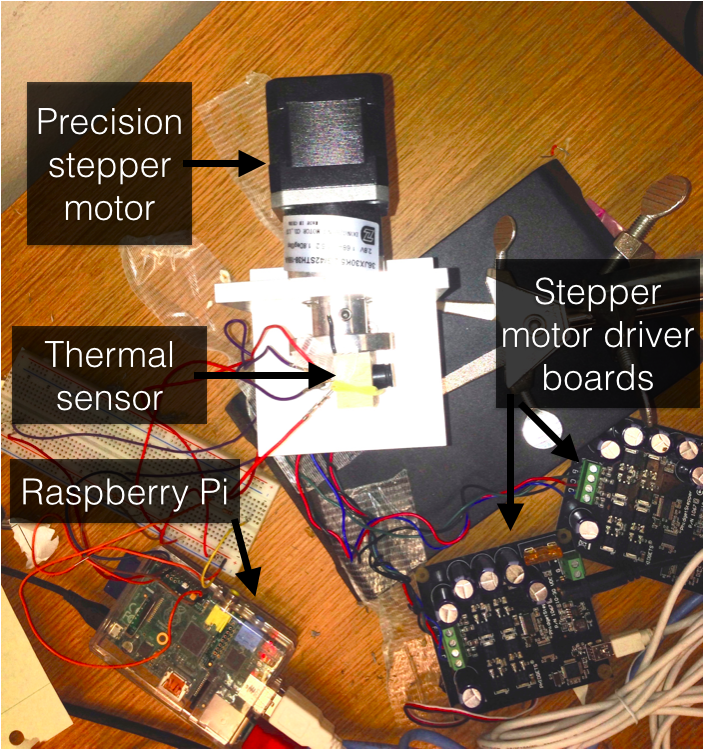
\includegraphics[width=0.9\textwidth]{figures/hardware-text}
%%\hspace{-1em}\captionof{figure}{Top-down view of hardware.}\label{hw}
%%\end{figure}
%\end{minipage}

\noindent We consider a multi-step sampling and refinement strategy, where subsequent steps focus samples onto (sub)regions of interest. Our overall approach is as follows. \\
\\
\underline{Initialize}: Let ${\cal I}^1$ be the whole image domain (e.g., $n^2$ virtual grid points overlaid on an $n\times n$ pixel scene), choose some $m \ll n^2$, and $\lambda > 0$.\\
\\
\underline{Iterate}: For $k=1,2,\dots,\log_2(n)-1$
\begin{itemize}
\item Randomly choose $m$ points $\Omega_k \subset {\cal I}^k$ (without replacement, and without duplicating previous choices) and collect $m$ samples $\mathbf{y}_k = \{y_{i,j}\}_{(i,j)\in\Omega_k}$
\item Reconstruct the image by enforcing sparsity in a \emph{partial} Haar wavelet basis.  Let $\mathbf{W}_{k+ 1}$ be a matrix whose columns are basis elements for the first (coarsest) $k+1$ levels of the Haar wavelet basis, and solve (e.g., using FISTA \cite{beck2009fast}):\vspace{-0.3em}
\begin{equation}\label{l1}
\hat{\mathbf{\theta}}_k = \arg \min_{\mathbf{\theta}} \|\mathbf{y} - \mathbf{W}_{k+1}\mathbf{\theta}\|_2^2 + \lambda \|\mathbf{\theta}\|_1  \vspace{-0.3em}
\end{equation}
 where $\mathbf{y}$ contains \emph{all} previously collected samples.
\item Identify coefficients of $\hat{\mathbf{\theta}}_k$ at the finest (i.e., $(k+1)$-st) scale that are ``significant''; let ${\cal I}^{k+1}$ be the grid points contained in the union of supports of those significant fine-scale coefficients.
\end{itemize}
The \emph{final} estimate is obtained by \eqref{l1} with $\mathbf{W}$ as the complete Haar basis.

          }
}

\headerbox{Hardware Platform}{name=implications1,column=1, below = recon, above=bottom}{
    \noindent \SSfontsize{Our overall design is based on independent two-dimensional actuation of single long-wavelength IR sensor$^*$, and was inspired by the \emph{Cheap Thermocam} project \cite{cheap} (as well as the Rice \emph{single-pixel} camera \cite{spc}). \\
    \\
    Highlights of our ($\approx$400\$) device:
    \begin{itemize}
    \item Two (individually controlled) stepper motors$^*$ steer the IR sensor toward points on a (finely-spaced) grid of points defined on the scene (see Figure~\ref{cam} below)
    \item Thermal sensor interfaced with a \emph{Raspberry Pi} (\emph{R-Pi}) via its I$^2$C serial bus; stepper motors interfaced with the R-Pi via USB. (See Figure~\ref{hw} below)
    \item The adaptive sampling-and-refinement algorithm (summarized above) is implemented directly on the R-Pi (in the \emph{Python} programming language).
    \end{itemize}


\begin{minipage}{0.48\textwidth}
%\begin{figure}[H]
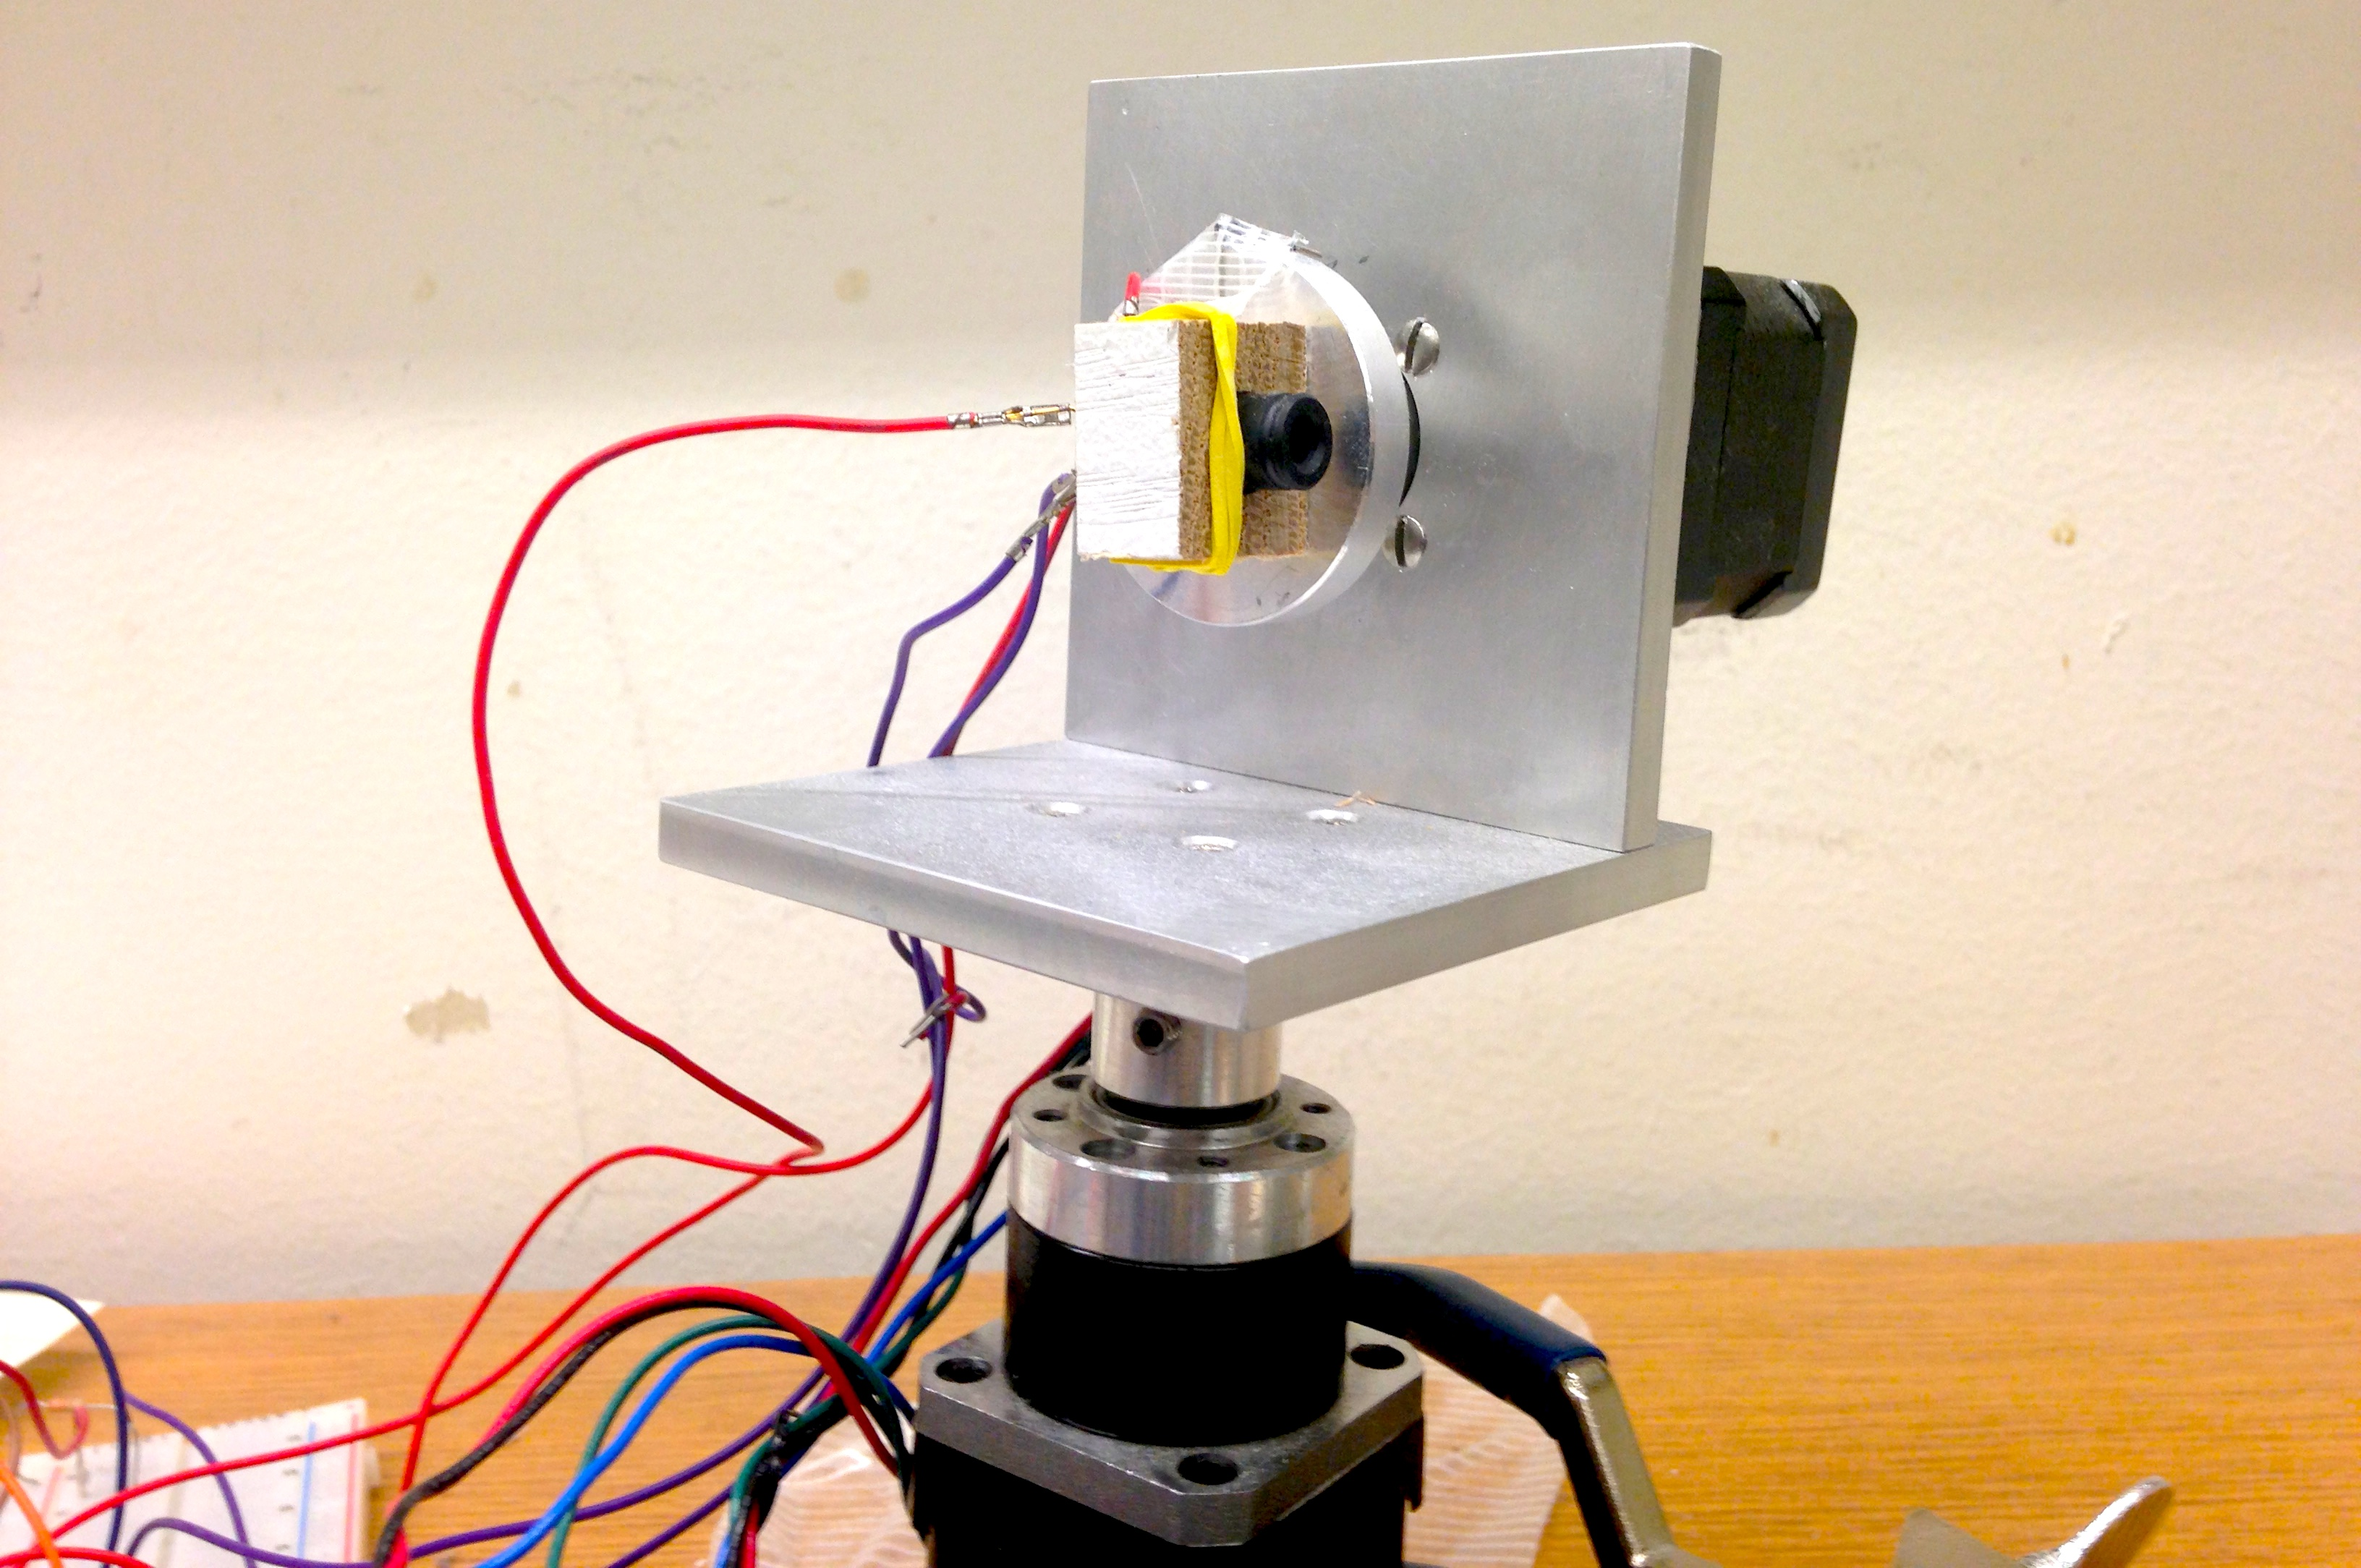
\includegraphics[width=0.95\textwidth]{figures/hardware_real}
\captionof{figure}{Image sensor and stepper motor assembly.}\label{cam}%\caption{\label{cam} The image sensor and stepper motor assembly.}
%\end{figure}
\end{minipage} \hspace{1em}
\begin{minipage}{0.45\textwidth}
%\begin{figure}
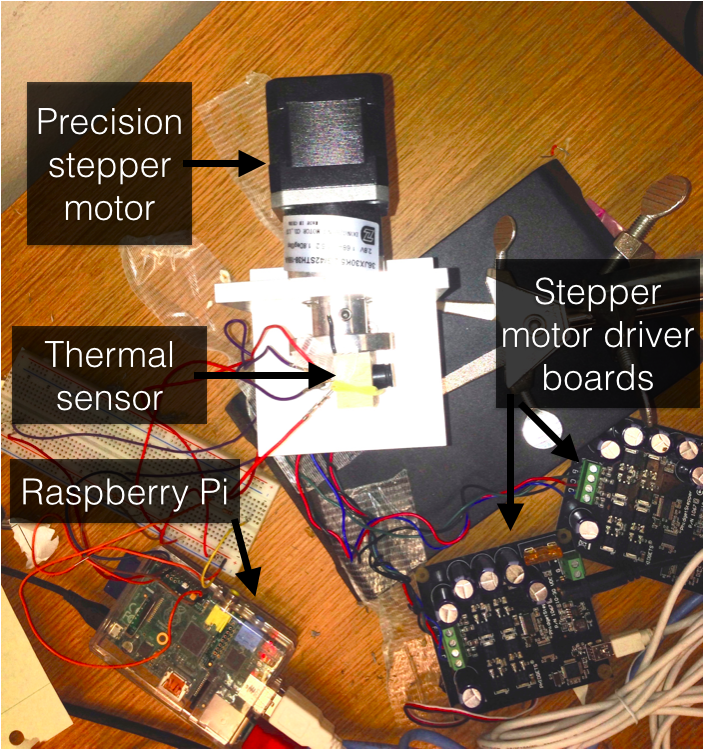
\includegraphics[width=0.9\textwidth]{figures/hardware-text}
\hspace{-1em}\captionof{figure}{Top-down view of hardware.}\label{hw}
%\end{figure}
\end{minipage}
\vspace{0.3em}

{\scriptsize $^*$We used the Melexis MLX90614 infrared sensor, and Phidgets stepper motors and driver boards. }

    }
}


  %%% COLUMN 3
%\headerbox{Hardware}{name=implications1,column=2}{%, row=0, below=top}{%, below = top, above=re}{
%    \noindent \SSfontsize{
%
%
%    \begin{minipage}{0.45\textwidth}
%This reconstruction algorithm was performed on actual hardware to demonstrate the use of this algorithm. It was performed on a Raspberry Pi credit card sized computer and used a single thermal sensor and precision stepper motors to collect data.
%\end{minipage}   \hspace{3em}
%    \begin{minipage}{0.45\textwidth}
%\begin{figure}[H]
%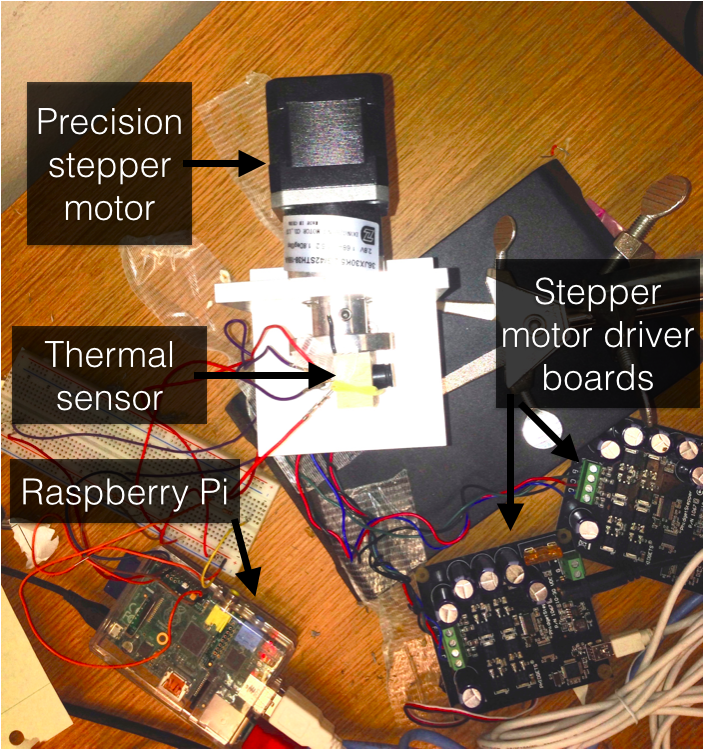
\includegraphics[width=0.80\textwidth]{figures/hardware-text}
%%\caption{\label{fig:blue_rectangle} Rectangle}
%\end{figure}
%\end{minipage}
%\vspace{1em}
%
%        %\begin{center}
%        %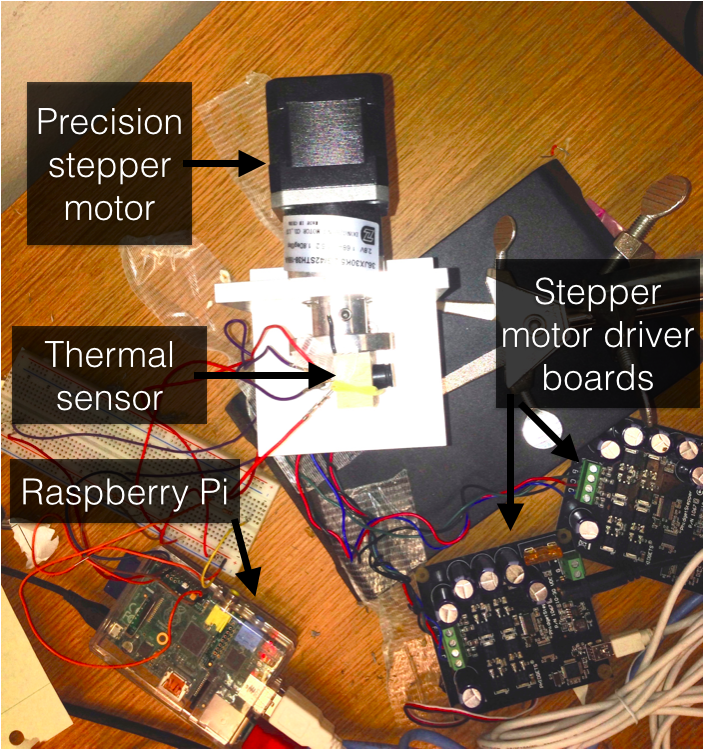
\includegraphics[width=0.45\textwidth]{figures/hardware-text}
%        %\end{center}
%
%%        \begin{center}
%%        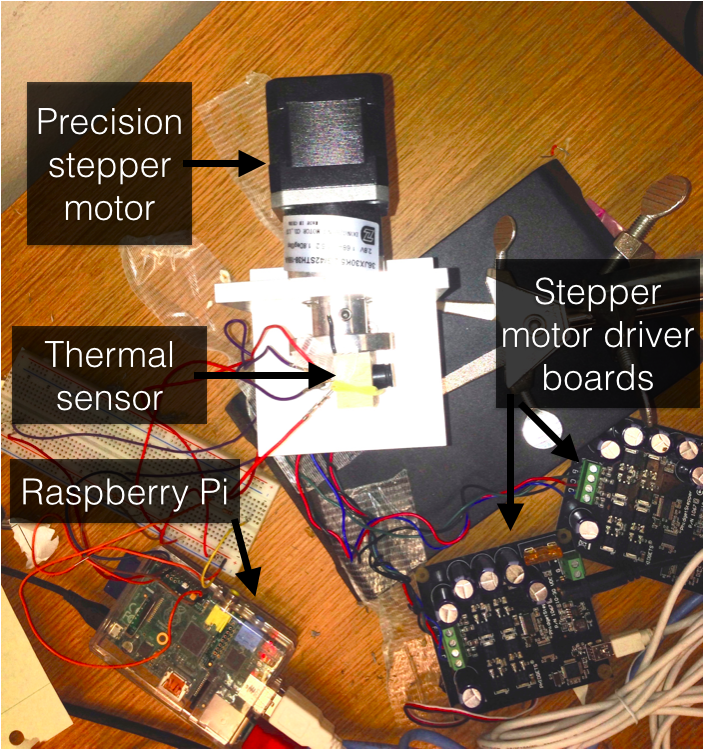
\includegraphics[width=0.30\textwidth]{figures/hardware-text}
%%        \end{center}
%    }
%    \vspace{0.0em}
%}
\headerbox{Experimental Evaluation}{name=exp,column=2}{%, below=implications1}{
    \noindent \SSfontsize{We evaluated our approach on a ``test scene'' comprised of a hot soldering iron against a concrete block-wall background.\\
    \\
    For $n\in\{64, 128, 256\}$ we virtually partitioned the scene into a $n\times n$ array of possible sampling locations, and compared the reconstructions obtained via \emph{exhaustive sampling} of all $n^2$ sampling points, and by the aforementioned adaptive sampling method.  A graphical comparison of the reconstructions for the $n=128$ case is provided below, along with a depiction of the sampling locations (determined automatically) using our adaptive sampling method.

        \begin{center}
        \begin{tabular}{ccc}
            True image & Our Reconstruction &  Adaptively \\
            (Exhaustive Sampling) & (Adaptive Sampling) & Sampled Locations \\
        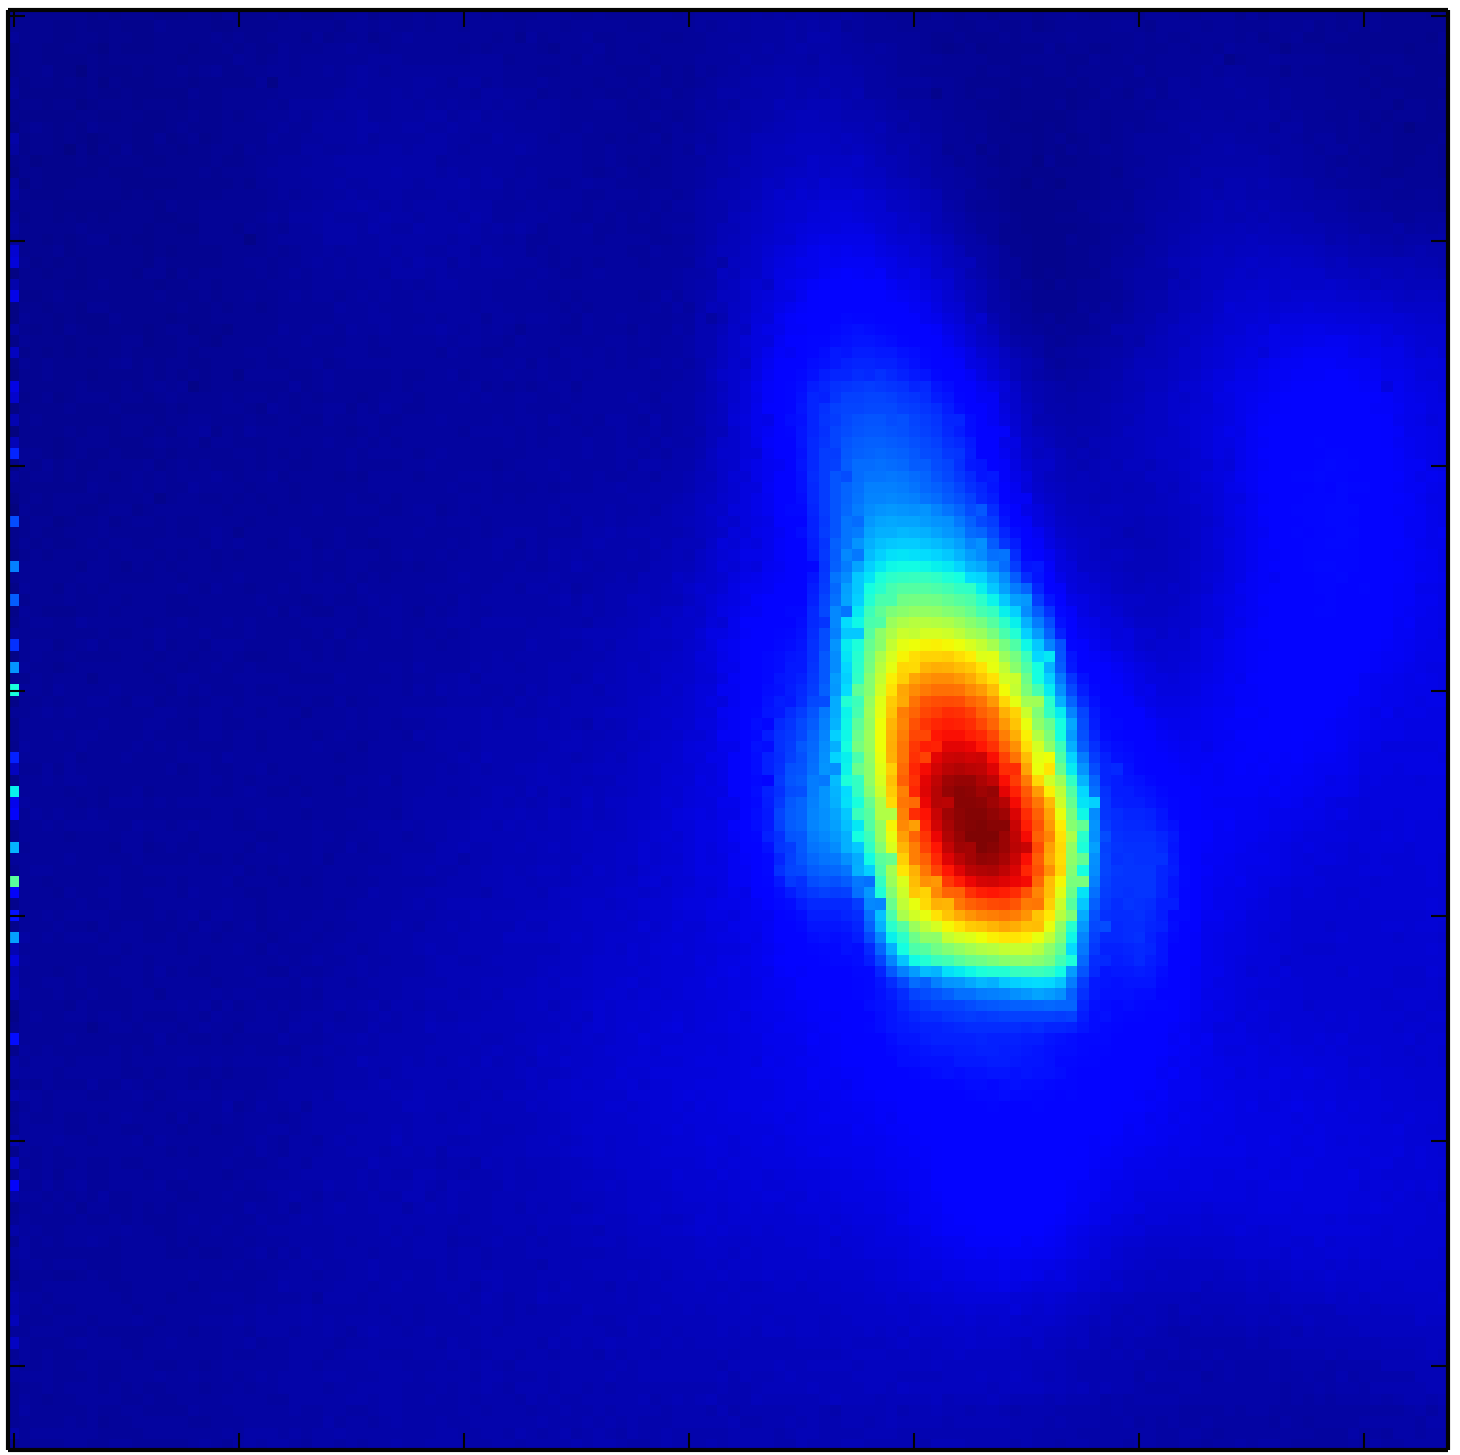
\includegraphics[width=0.21\textwidth]{figures/results/thermal/2014-09-09thermal_x}&
        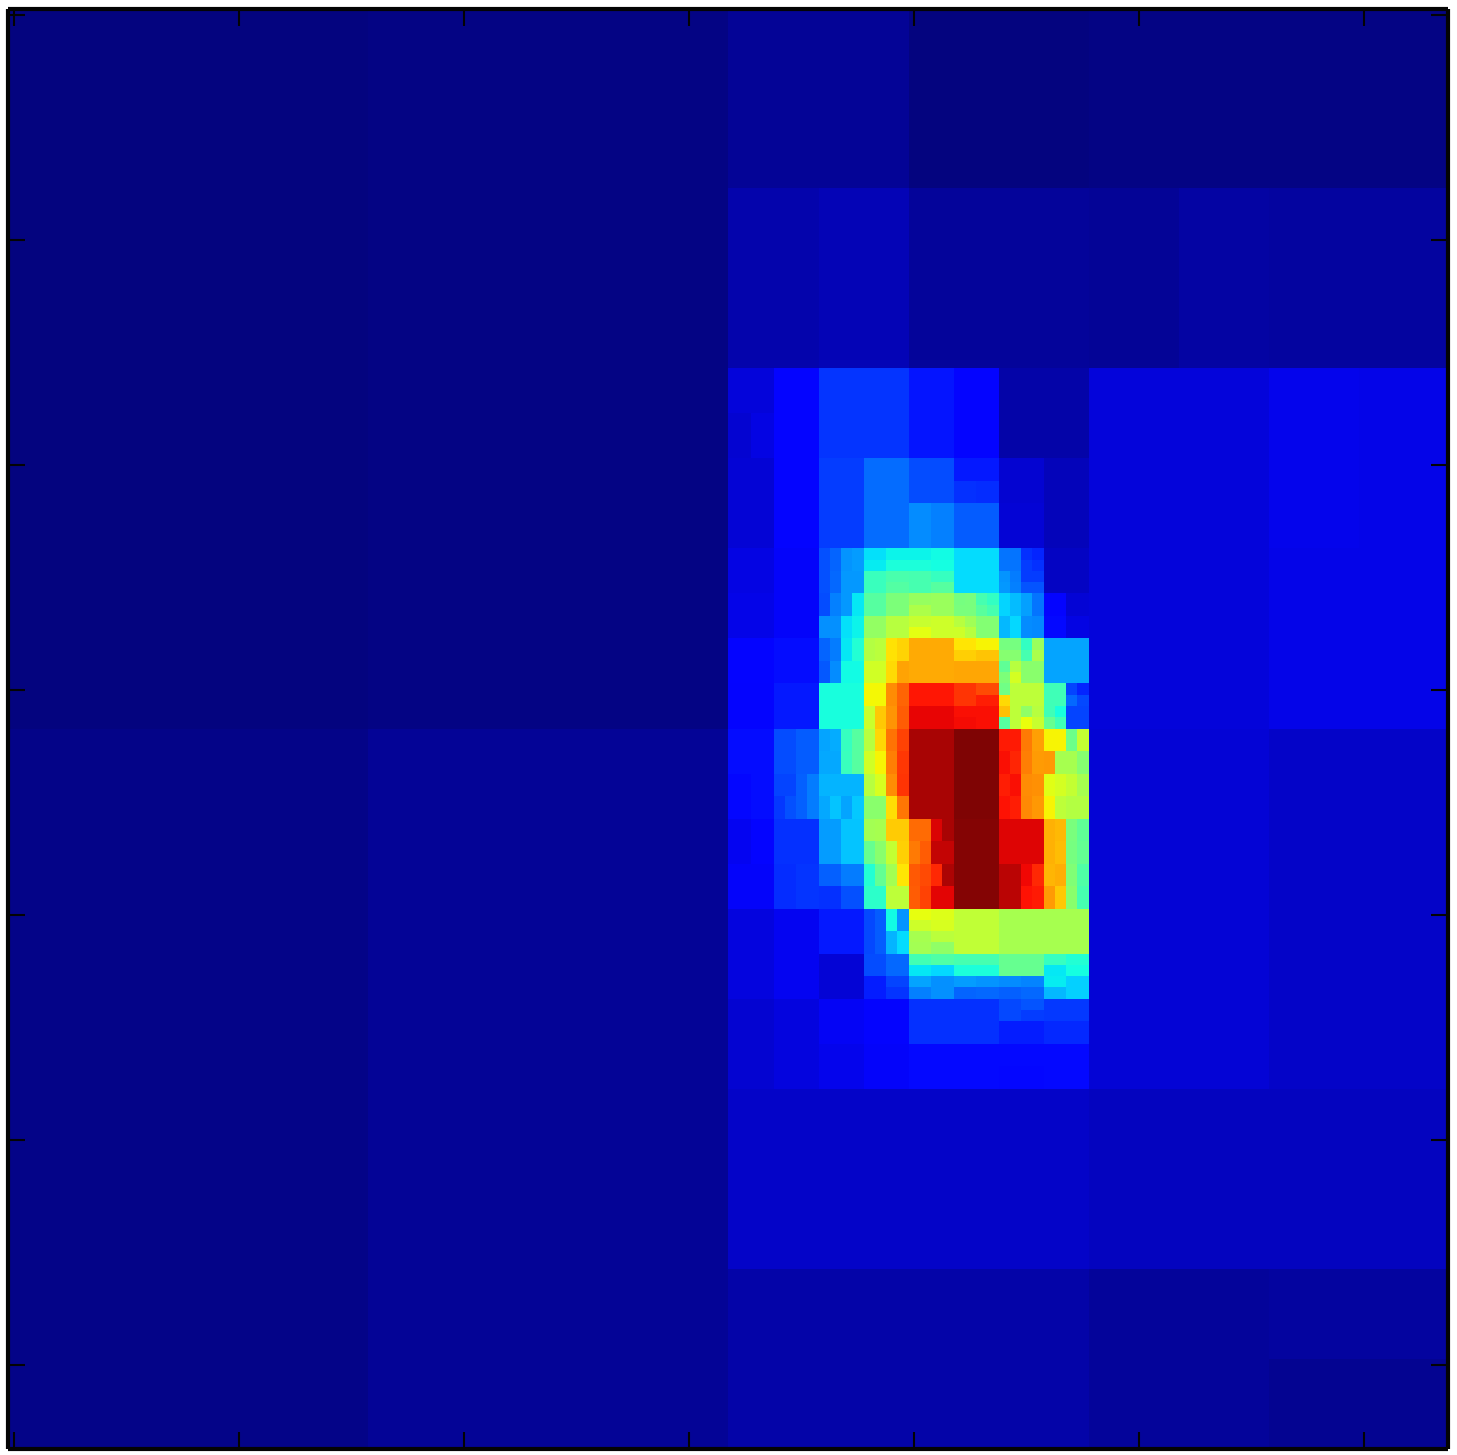
\includegraphics[width=0.21\textwidth]{figures/results/thermal/2014-09-09thermal_xhat}&
        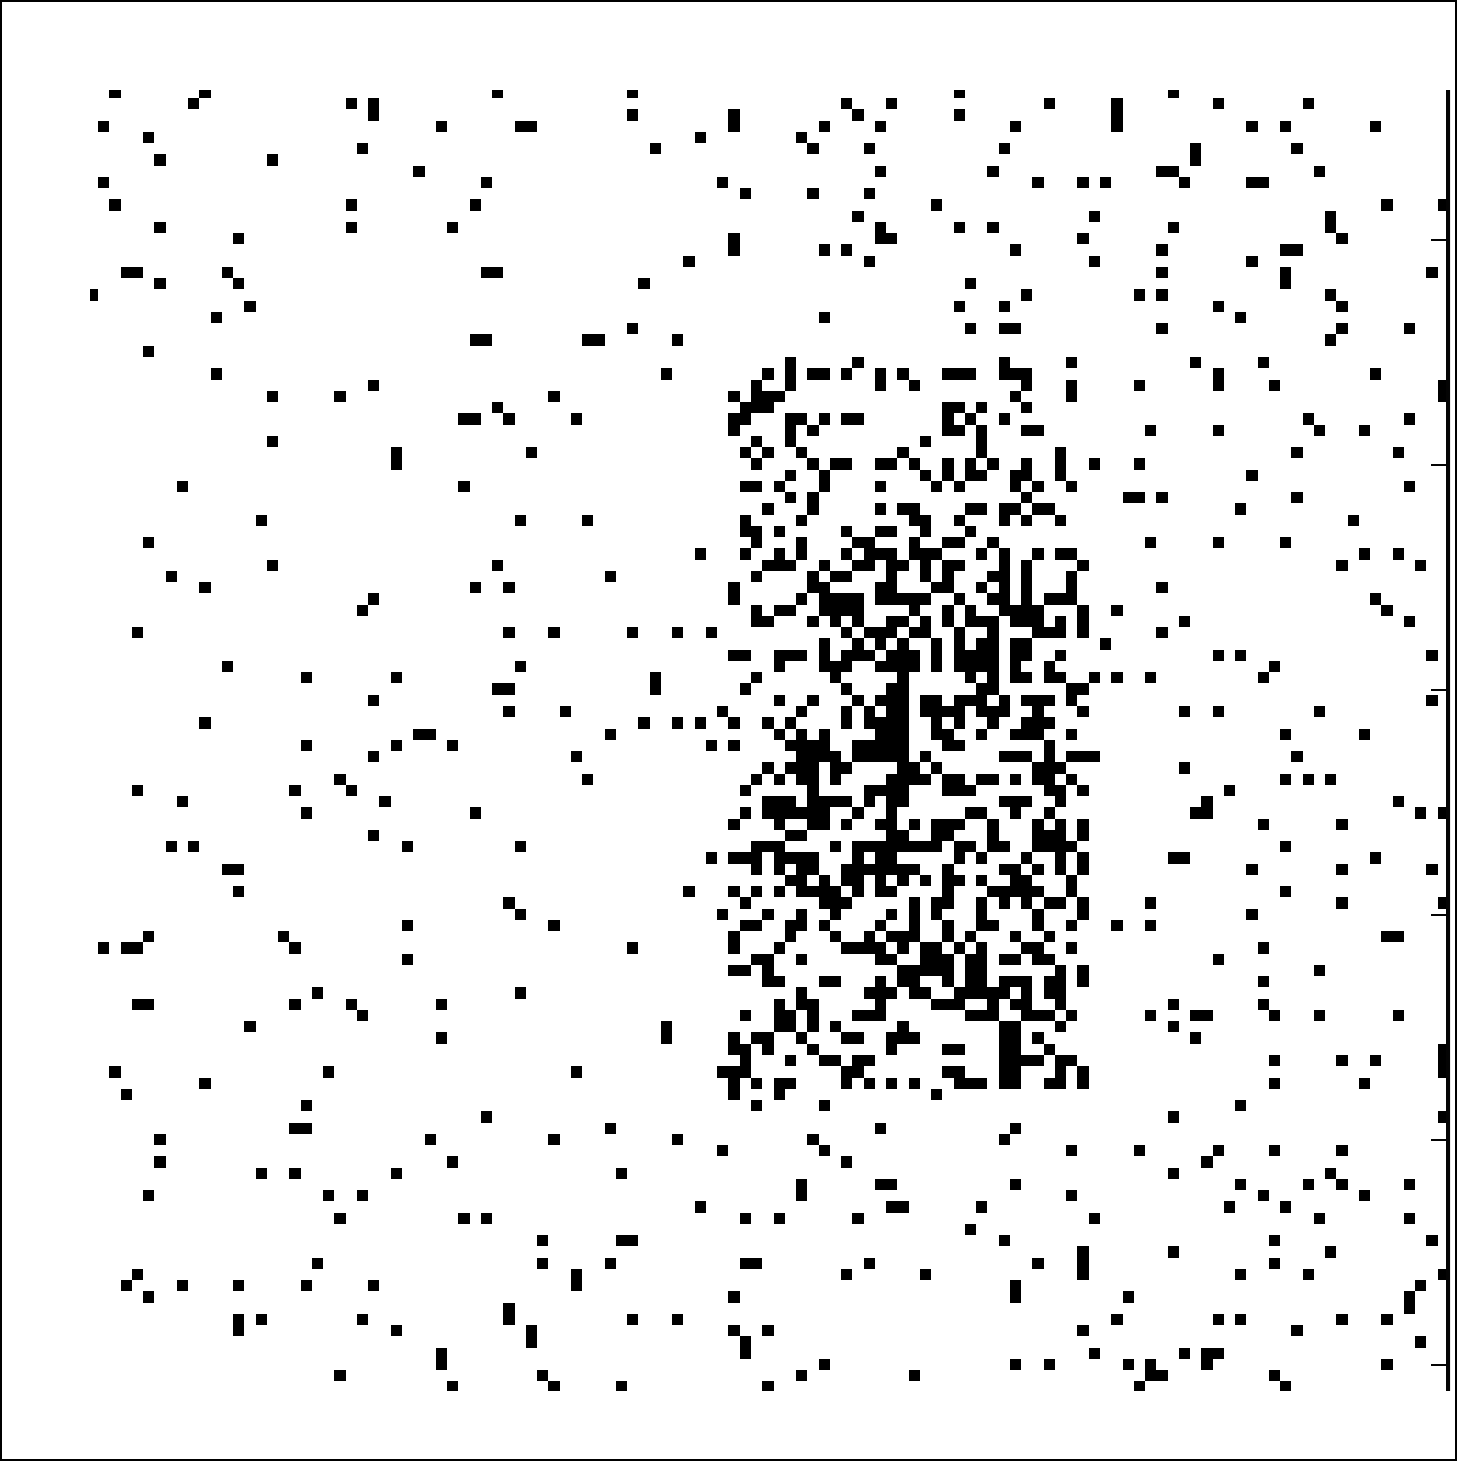
\includegraphics[width=0.21\textwidth]{figures/python_scripting/thermal_sampleAt}\\
        \end{tabular}
        \end{center}

\noindent We also tabulated the image acquisition time for each approach (shown below).  Overall, we see that the adaptive sensing approach yields $10\times$ or more improvements in acquisition time.

        \begin{center}
        \begin{tabular}{c|cc}
            % adaptive: t= 1.3 * 46e-3 * n^2 * 8.8/(100*60)
            % exhaustive: t= 46e-3 * n^2 / 60
             & Exhaustive & Adaptive\\
            Image dimension  & Sampling Time (min) & Sampling Time (min)\\
            \hline
            %$n=64$ & 0.36 & 3.14 \\
            %$n=128$ & 1.43 & 12.56\\
            %$n=256$ & 5.74 & 50.244\\
            $n=64$ & 3.14 & 0.36 \\
            $n=128$ &  12.56 & 1.43 \\
            $n=256$ & 50.244 & 5.74 \\

        \end{tabular}
        \end{center}
    }
    \vspace{0.0em}
}

\headerbox{Conclusions \& Next Steps}{name=next,column=2,below=exp}{
    \noindent \SSfontsize{We demonstrated (experimentally) the viability of a novel, low-cost ``single pixel'' adaptive sampling thermal device for long-wavelength infrared (thermal) imaging.\\
    \\
        Ongoing extensions to this initial effort include:
        \begin{itemize}
        \item establishing rigorous justification for our sensing strategy (e.g., using analyses along the lines of \cite{Nowak}), and
        \item implementing sampling-path planning strategies designed to minimize the acquisition time at each sampling step.
        \end{itemize}
        We also plan to investigate extensions of this basic architecture to other single-sensor imaging problems (e.g., terahertz imaging?).

        }
}
\headerbox{References \& Acknowledgments}{name=references,column=2,below=next, above=bottom}{\vfill
    \renewcommand{\section}[2]{}
    \bibliographystyle{ieee}
    {\scriptsize \bibliography{refs}}
       %\vspace{-1em}
     \noindent  {\SSfontsize The authors graciously acknowledge support from The University of Minnesota.}
}
%\headerbox{Acknowledgement}{name=source code,column=2,above=bottom, below = references}{
%    \noindent \scriptsize{This work was supported by  NSF Award XXX-YYYYYYY.}
%
%    \vspace{0em}
%}

\end{poster}

\end{document}
